\documentclass[a4paper,10pt]{article}

\usepackage{amsmath}
\usepackage{float}
\usepackage{graphicx}
\usepackage{tikz,ifthen}
\usetikzlibrary{calc}
\usepackage[toc, acronym]{glossaries}
\usepackage{hyperref}
\usepackage[toc, acronym]{glossaries}

\hypersetup{colorlinks=true, linkcolor=black}

\newacronym{lgca}{LGCA}{Lattice-Gas Cellular Automata}
\newacronym{lbm}{LBM}{lattice Boltzmann models}
\newtheorem{theorem}{Theorem}[section]
\newtheorem{lemma}[theorem]{Lemma}
\newtheorem{proposition}[theorem]{Proposition}
\newtheorem{corollary}[theorem]{Corollary}
\newenvironment{definition}[1][Definition]{\begin{trivlist}
\item[\hskip \labelsep {\bfseries #1}]}{\end{trivlist}}

\author{Mr. S. Schreiber}
\date{\today}
\title{Flow modelling with lattice gas cellular automata}
%glossary entries
\newglossaryentry{EP}
{
	name = {pauli exclusion principle},
	description={is the quantum mechanical principle that no 			two identical fermions may occupy the same quantum state 			simultaneously.}
}


\begin{document}
\maketitle
\begin{abstract}
The use of lattice in flow modelling has become increasingly popular over the last couple of decades and during that time a lot of models have been developed. We'll be investigating three of the more widely used models i.e. FHP and \acrshort{lbm}. The following will be discussed for each model: history, assumptions, the collision rules, the propagation rules, calculation of the mass and momentum density, time complexity analysis, applications, defects and does it obey the desired hydrodynamics equation (Navier Stokes) in the macroscopic limit. 
\end{abstract}
\section{Introduction}

\section{Background}
\subsection{Cellular automata}
Informally a cellular automaton is a system made up of many discrete cells, usually a M by N grid. Each one of these cells can be in one of a finite number of states. Each cell or automaton may only change state on a fixed interval and only according to a fixed set of rules. These rules depend on the cells own value and that of this neighbours. A cellular automaton can formally be defined by
\begin{definition}
A cellular automaton is a 4-tuple, $C = \{S,s_{0},f,G\}$, where
\begin{enumerate}
\item $S$ is a finite set of state,
\item $s_{0}$ is the initial state,
\item $G$ is the neighbourhood,
\item $f:S^{n} \rightarrow S$.
\end{enumerate}
\end{definition}
Two popular neighbourhoods are the von Neumann and Moore.
The von Neumann neighbourhood for range r can be defined by \[ G_{(x_{0}, y_{0})} = \{(x, y): \left|x - x_{0} \right| + \left|y - y_{0}\right| \leq r\}.\]
The Moore neighbourhood for range r can be defined by \[ G_{(x_{0}, y_{0})} = \{(x, y): \left|x - x_{0}\right| \leq r, \left|y - y_{0}\right| \leq r \}.\]
A popular example of a cellular automata that makes use of a Moore neighbourhood with r = 1 is ``Conway's game of life''.
\subsection{Lattice gas cellular automata}
Lattice gas cellular automata is a cellular automata where the transition functions $f$ is split into two phases i.e. propagation phase and collision phase. Also each cell has n number of local sites, where n is the number of directly connected neighbours. Each site is associated with a specific velocity vector $\textbf{c}_{i}$ $( i = 0,1,2,\dots,n)$. Velocity vectors are the edge's between cells and their neighbours and is of unit length. Sites may be empty or occupied by at most one particle. This \gls{EP} is characteristic for all lattice-gas cellular automata.   
\begin{figure}[H]
  \centering
  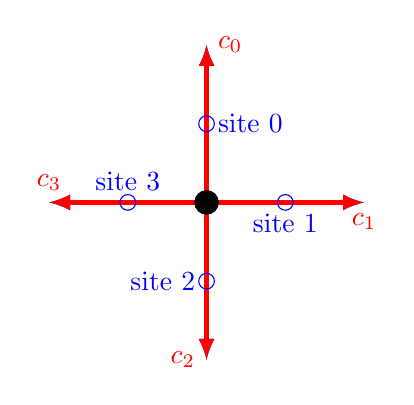
\begin{tikzpicture}

    \coordinate (Origin) at (0,0);
    \coordinate (site1) at (0,2);
    \coordinate (site2) at (2,0);
    \coordinate (site3) at (0,-2);
    \coordinate (site4) at (-2,0);  
    
    \draw [ultra thick,-latex,blue] (Origin)
        -- (site1) node [midway, right] {site 0};
    \draw [ultra thick,-latex,blue] (Origin)
        -- (site2) node [midway,below] {site 1};
    \draw [ultra thick,-latex,blue] (Origin)
        -- (site3) node [midway,left] {site 2};
    \draw [ultra thick,-latex,blue] (Origin)
        -- (site4) node [midway,above] {site 3};
        
	\draw [ultra thick,-latex,red] (Origin)
        -- (site1) node [right] {$c_0$};
    \draw [ultra thick,-latex,red] (Origin)
        -- (site2) node [below] {$c_1$};
    \draw [ultra thick,-latex,red] (Origin)
        -- (site3) node [left] {$c_2$};
    \draw [ultra thick,-latex,red] (Origin)
        -- (site4) node [above] {$c_3$};
       
    \node[draw,circle,inner sep=3pt,fill] at (0,0) {};
    \node[draw,circle,inner sep=2pt,blue] at (1,0) {};
	\node[draw,circle,inner sep=2pt,blue] at (0,1) {};
	\node[draw,circle,inner sep=2pt,blue] at (-1,0) {};
	\node[draw,circle,inner sep=2pt,blue] at (0,-1) {};
  \end{tikzpicture}
  \caption{Here is an example of a single cell with 4 velocity vectors and 4 empty sites.}
  \label{figure:single-cell}
\end{figure}
\noindent As previously mentioned the transition function $f$ is divided into two phases propagation and collision.
The collision phase only applies rules that act on a single cell i.e. the local sites.
The propagation phase on the other hand applies rules between cells. What those rules are will vary between implementations and will be discussed later.

\section{\acrfull{lgca}}
\subsection{HPP}
\subsubsection{History}
The HPP model was proposed by Hardy, de Pazzis and Pomeau in 1973.
This was the first \acrshort{lgca} model and received its name from the initials of the authors. It is the simplest \acrshort{lgca} model and is only mentioned for its historical importance and not for its application because it does not lead to the Navier-Stokes equation in the macroscopic limit. 
\subsubsection{Model Description}
The HPP model is a \acrshort{lgca} that make use of a square lattice.
Each cell has 4 velocity vectors $\textbf{c}_{i}$ where $i \in \{0, 1, 2, 3\}$. Each velocity vector is associated with one site, see Fig \ref{figure:single-cell}. All particles have the same mass m and are indistinguishable. A site can only be in one of two states occupied or empty. A site can not be occupied by more than one particle (\Gls{EP}). It will lead to equilibrium distributions of Fermi-Dirac type for
the mean occupation of the cells.%Cite this
The two phase will now be discussed.
\subsubsection{Collision phase}
This is a basic model and thus only has one collision rule, all other configurations are treated as if no collisions have occurred. The collision rules only consider local sites and only has a local effect. The notation to select the nth site is $s_{n}$. If $s_{i}$ is equals to the opposite site $s_{j}$ where $j = (i + 2)\bmod{4}$ and the other two sites are empty. Then $s_{k}$ will take the value of $s_{i}$ and $s_{d}$ will take the value of $s_{j}$ where k and d are the indices of the open sites. The sites $s_{j}$ and $s_{i}$ are then set to empty.
\begin{figure}[H]
\begin{minipage}[width=0.5\linewidth]{0.5\textwidth}
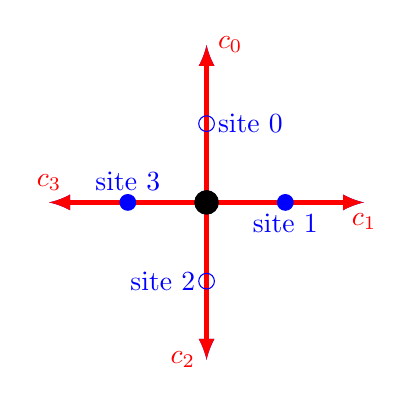
\begin{tikzpicture}
    \coordinate (Origin) at (0,0);
    \coordinate (site1) at (0,2);
    \coordinate (site2) at (2,0);
    \coordinate (site3) at (0,-2);
    \coordinate (site4) at (-2,0);  
    
    \draw [ultra thick,-latex,blue] (Origin)
        -- (site1) node [midway, right] {site 0};
    \draw [ultra thick,-latex,blue] (Origin)
        -- (site2) node [midway,below] {site 1};
    \draw [ultra thick,-latex,blue] (Origin)
        -- (site3) node [midway,left] {site 2};
    \draw [ultra thick,-latex,blue] (Origin)
        -- (site4) node [midway,above] {site 3};
        
	\draw [ultra thick,-latex,red] (Origin)
        -- (site1) node [right] {$c_0$};
    \draw [ultra thick,-latex,red] (Origin)
        -- (site2) node [below] {$c_1$};
    \draw [ultra thick,-latex,red] (Origin)
        -- (site3) node [left] {$c_2$};
    \draw [ultra thick,-latex,red] (Origin)
        -- (site4) node [above] {$c_3$};
       
    \node[draw,circle,inner sep=3pt,fill] at (0,0) {};
    \node[draw,circle,inner sep=2pt,fill,blue] at (1,0) {};
	\node[draw,circle,inner sep=2pt,blue] at (0,1) {};
	\node[draw,circle,inner sep=2pt,fill,blue] at (-1,0) {};
	\node[draw,circle,inner sep=2pt,blue] at (0,-1) {};
  \end{tikzpicture}
  \caption{Before Collision}
  \label{figure:collision_HPP1}
\end{minipage} 
\begin{minipage}[width=0.5\linewidth]{0.5\textwidth}
 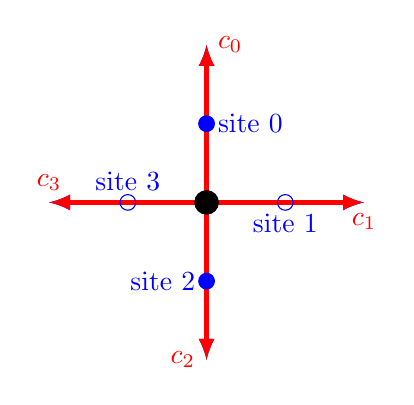
\begin{tikzpicture}
    \coordinate (Origin) at (0,0);
    \coordinate (site1) at (0,2);
    \coordinate (site2) at (2,0);
    \coordinate (site3) at (0,-2);
    \coordinate (site4) at (-2,0);  
    
    \draw [ultra thick,-latex,blue] (Origin)
        -- (site1) node [midway, right] {site 0};
    \draw [ultra thick,-latex,blue] (Origin)
        -- (site2) node [midway,below] {site 1};
    \draw [ultra thick,-latex,blue] (Origin)
        -- (site3) node [midway,left] {site 2};
    \draw [ultra thick,-latex,blue] (Origin)
        -- (site4) node [midway,above] {site 3};
        
	\draw [ultra thick,-latex,red] (Origin)
        -- (site1) node [right] {$c_0$};
    \draw [ultra thick,-latex,red] (Origin)
        -- (site2) node [below] {$c_1$};
    \draw [ultra thick,-latex,red] (Origin)
        -- (site3) node [left] {$c_2$};
    \draw [ultra thick,-latex,red] (Origin)
        -- (site4) node [above] {$c_3$};
       
    \node[draw,circle,inner sep=3pt,fill] at (0,0) {};
    \node[draw,circle,inner sep=2pt,blue] at (1,0) {};
	\node[draw,circle,inner sep=2pt,fill,blue] at (0,1) {};
	\node[draw,circle,inner sep=2pt,blue] at (-1,0) {};
	\node[draw,circle,inner sep=2pt,fill,blue] at (0,-1) {};
  \end{tikzpicture}
  \caption{After Collision}
  \label{figure:collision_HPP2}
\end{minipage} 
\end{figure}
\subsubsection{Propagation phase}
The propagation phase only considers the local neighbours of a cell and not the cell it self. The propagation phase has no effect on the local neighbours of a cell, only on the cell it self. A thing to keep in mind while applying the propagation phase that it will require two states/matrices one that stores the previous results and one that will store the new results.

\begin{figure}[H]
\begin{minipage}{0.5\textwidth}
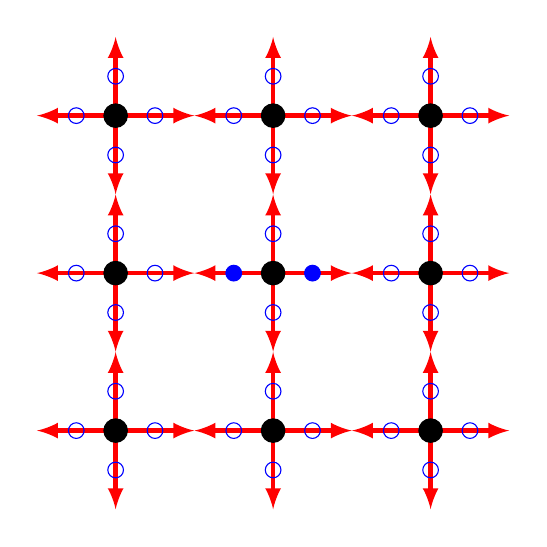
\begin{tikzpicture}[scale=0.50]
\foreach \x in {-4, 0, 4}
	{
	\foreach \y in {-4, 0, 4}
		{
		\ifthenelse{\x = 0 \AND \y = 0}{
    		\coordinate (Origin) at (0 + \x, 0 + \y);
    		\coordinate (site1) at (0+ \x,2+ \y);
    		\coordinate (site2) at (2+ \x,0+ \y);
    		\coordinate (site3) at (0+ \x,-2+ \y);
    		\coordinate (site4) at (-2+ \x,0+ \y);  
    
 
        
		\draw [ultra thick,-latex,red] (Origin)
   		     -- (site1) node [right] {};
    		\draw [ultra thick,-latex,red] (Origin)
        		-- (site2) node [below] {};
    		\draw [ultra thick,-latex,red] (Origin)
        		-- (site3) node [left] {};
    		\draw [ultra thick,-latex,red] (Origin)
        		-- (site4) node [above] {};
       
    		\node[draw,circle,inner sep=3pt,fill] at (0+ \x,0+ \y) {};
    		\node[draw,circle,inner sep=2pt,fill,blue] at (1+ \x,0+ \y) {};
		\node[draw,circle,inner sep=2pt,blue] at (0+ \x,1+ \y) {};
		\node[draw,circle,inner sep=2pt,fill,blue] at (-1+ \x,0+ \y) {};
		\node[draw,circle,inner sep=2pt,blue] at (0+ \x,-1+ \y) {};
		}%else
		{
		
    		\coordinate (Origin) at (0 + \x, 0 + \y);
    		\coordinate (site1) at (0+ \x,2+ \y);
    		\coordinate (site2) at (2+ \x,0+ \y);
    		\coordinate (site3) at (0+ \x,-2+ \y);
    		\coordinate (site4) at (-2+ \x,0+ \y);  
    

        
		\draw [ultra thick,-latex,red] (Origin)
   		     -- (site1) node [right] {};
    		\draw [ultra thick,-latex,red] (Origin)
        		-- (site2) node [below] {};
    		\draw [ultra thick,-latex,red] (Origin)
        		-- (site3) node [left] {};
    		\draw [ultra thick,-latex,red] (Origin)
        		-- (site4) node [above] {};
       
    		\node[draw,circle,inner sep=3pt,fill] at (0+ \x,0+ \y) {};
    		\node[draw,circle,inner sep=2pt,blue] at (1+ \x,0+ \y) {};
		\node[draw,circle,inner sep=2pt,blue] at (0+ \x,1+ \y) {};
		\node[draw,circle,inner sep=2pt,blue] at (-1+ \x,0+ \y) {};
		\node[draw,circle,inner sep=2pt,blue] at (0+ \x,-1+ \y) {};
		}
		}
	}
  \end{tikzpicture}
   
  \caption{Initial configuration, before collision}
  \label{figure:collision_HPP3} 
   \end{minipage}
\begin{minipage}{0.5\textwidth}
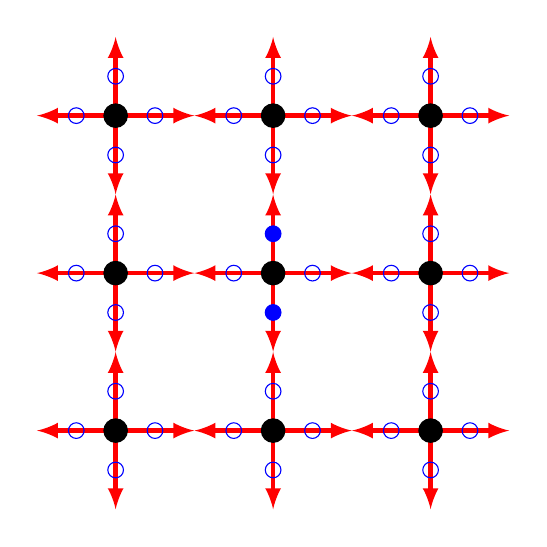
\begin{tikzpicture}[scale=0.50]
\foreach \x in {-4, 0, 4}
	{
	\foreach \y in {-4, 0, 4}
		{
		\ifthenelse{\x = 0 \AND \y = 0}{
    		\coordinate (Origin) at (0 + \x, 0 + \y);
    		\coordinate (site1) at (0+ \x,2+ \y);
    		\coordinate (site2) at (2+ \x,0+ \y);
    		\coordinate (site3) at (0+ \x,-2+ \y);
    		\coordinate (site4) at (-2+ \x,0+ \y);  
        
		\draw [ultra thick,-latex,red] (Origin)
   		     -- (site1) node [right] {};
    		\draw [ultra thick,-latex,red] (Origin)
        		-- (site2) node [below] {};
    		\draw [ultra thick,-latex,red] (Origin)
        		-- (site3) node [left] {};
    		\draw [ultra thick,-latex,red] (Origin)
        		-- (site4) node [above] {};
       
    		\node[draw,circle,inner sep=3pt,fill] at (0+ \x,0+ \y) {};
    		\node[draw,circle,inner sep=2pt,blue] at (1+ \x,0+ \y) {};
		\node[draw,circle,inner sep=2pt,fill,blue] at (0+ \x,1+ \y) {};
		\node[draw,circle,inner sep=2pt,blue] at (-1+ \x,0+ \y) {};
		\node[draw,circle,inner sep=2pt,fill,blue] at (0+ \x,-1+ \y) {};
		}%else
		{
		
    		\coordinate (Origin) at (0 + \x, 0 + \y);
    		\coordinate (site1) at (0+ \x,2+ \y);
    		\coordinate (site2) at (2+ \x,0+ \y);
    		\coordinate (site3) at (0+ \x,-2+ \y);
    		\coordinate (site4) at (-2+ \x,0+ \y);  
        
		\draw [ultra thick,-latex,red] (Origin)
   		     -- (site1) node [right] {};
    		\draw [ultra thick,-latex,red] (Origin)
        		-- (site2) node [below] {};
    		\draw [ultra thick,-latex,red] (Origin)
        		-- (site3) node [left] {};
    		\draw [ultra thick,-latex,red] (Origin)
        		-- (site4) node [above] {};
       
    		\node[draw,circle,inner sep=3pt,fill] at (0+ \x,0+ \y) {};
    		\node[draw,circle,inner sep=2pt,blue] at (1+ \x,0+ \y) {};
		\node[draw,circle,inner sep=2pt,blue] at (0+ \x,1+ \y) {};
		\node[draw,circle,inner sep=2pt,blue] at (-1+ \x,0+ \y) {};
		\node[draw,circle,inner sep=2pt,blue] at (0+ \x,-1+ \y) {};
		}
		}
	}
  \end{tikzpicture}
  \caption{After Collision and before propagation}
  \label{figure:propagation_HPP1} 
   \end{minipage}
   \begin{minipage}{0.5\textwidth}
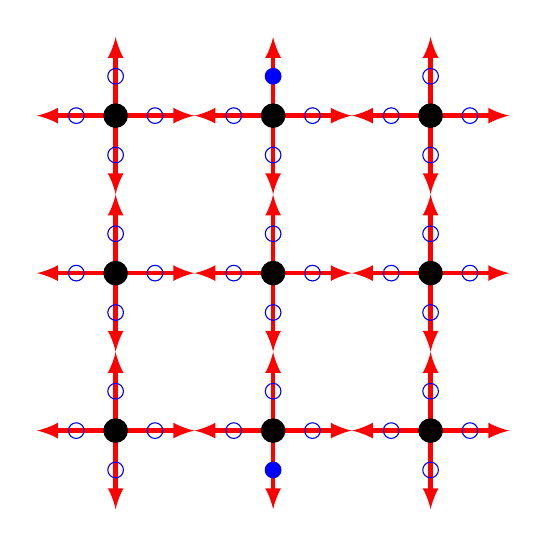
\begin{tikzpicture}[scale=0.50]
\foreach \x in {-4, 0, 4}
	{
	\foreach \y in {-4, 0, 4}
		{
		\ifthenelse{\x = 0 \AND \y = -4}{
    			\coordinate (Origin) at (0 + \x, 0 + \y);
    			\coordinate (site1) at (0+ \x,2+ \y);
    			\coordinate (site2) at (2+ \x,0+ \y);
    			\coordinate (site3) at (0+ \x,-2+ \y);
    			\coordinate (site4) at (-2+ \x,0+ \y);  
        
			\draw [ultra thick,-latex,red] (Origin)
   			     -- (site1) node [right] {};
    			\draw [ultra thick,-latex,red] (Origin)
        			-- (site2) node [below] {};
    			\draw [ultra thick,-latex,red] (Origin)
        			-- (site3) node [left] {};
    			\draw [ultra thick,-latex,red] (Origin)
        			-- (site4) node [above] {};
       
    			\node[draw,circle,inner sep=3pt,fill] at (0+ \x,0+ \y) {};
    			\node[draw,circle,inner sep=2pt,blue] at (1+ \x,0+ \y) {};
			\node[draw,circle,inner sep=2pt,blue] at (0+ \x,1+ \y) {};
			\node[draw,circle,inner sep=2pt,blue] at (-1+ \x,0+ \y) {};
			\node[draw,circle,inner sep=2pt,fill,blue] at (0+ \x,-1+ \y) {};
		}%else
		{
			\ifthenelse{\x = 0 \AND \y = 4}
				{
    					\coordinate (Origin) at (0 + \x, 0 + \y);
    					\coordinate (site1) at (0+ \x,2+ \y);
    					\coordinate (site2) at (2+ \x,0+ \y);
    					\coordinate (site3) at (0+ \x,-2+ \y);
    					\coordinate (site4) at (-2+ \x,0+ \y);  
        
					\draw [ultra thick,-latex,red] (Origin)
   					     -- (site1) node [right] {};
    					\draw [ultra thick,-latex,red] (Origin)
       	 				-- (site2) node [below] {};
    					\draw [ultra thick,-latex,red] (Origin)
       	 				-- (site3) node [left] {};
    					\draw [ultra thick,-latex,red] (Origin)
        					-- (site4) node [above] {};
       
    					\node[draw,circle,inner sep=3pt,fill] at (0+ \x,0+ \y) {};
    					\node[draw,circle,inner sep=2pt,blue] at (1+ \x,0+ \y) {};
					\node[draw,circle,inner sep=2pt,fill,blue] at (0+ \x,1+ \y) {};
					\node[draw,circle,inner sep=2pt,blue] at (-1+ \x,0+ \y) {};
					\node[draw,circle,inner sep=2pt,blue] at (0+ \x,-1+ \y) {};
				}% else
				{
					\coordinate (Origin) at (0 + \x, 0 + \y);
    					\coordinate (site1) at (0+ \x,2+ \y);
    					\coordinate (site2) at (2+ \x,0+ \y);
    					\coordinate (site3) at (0+ \x,-2+ \y);
    					\coordinate (site4) at (-2+ \x,0+ \y);  
        
					\draw [ultra thick,-latex,red] (Origin)
   					     -- (site1) node [right] {};
    					\draw [ultra thick,-latex,red] (Origin)
       	 				-- (site2) node [below] {};
    					\draw [ultra thick,-latex,red] (Origin)
       	 				-- (site3) node [left] {};
    					\draw [ultra thick,-latex,red] (Origin)
        					-- (site4) node [above] {};
       
    					\node[draw,circle,inner sep=3pt,fill] at (0+ \x,0+ \y) {};
    					\node[draw,circle,inner sep=2pt,blue] at (1+ \x,0+ \y) {};
					\node[draw,circle,inner sep=2pt,blue] at (0+ \x,1+ \y) {};
					\node[draw,circle,inner sep=2pt,blue] at (-1+ \x,0+ \y) {};
					\node[draw,circle,inner sep=2pt,blue] at (0+ \x,-1+ \y) {};
				}
			}
		}
	}
  \end{tikzpicture}
  \caption{After propagation}
  \label{figure:propagation_HPP2} 
   \end{minipage}
\end{figure}
\subsubsection{Boundry conditions}
\subsubsection{Mass and Momentum Densities}
\subsubsection{Time complexity analysis}
\subsubsection{Applications}
\subsubsection{defects}
Due to 
\subsection{FHP}
\subsubsection{History}
The FHP model was proposed by Frisch, Hasslacher and Pomeau in 1986 and received its name from the initials of the authors. This was the first model that showed it is possible for a \acrshort{lgca} to yield the Navier-Stokes equation in the macroscopic limit. This was a big discovery and lead to the rapid development of lattice-gas cellular automata. There where three FHP models developed FHP-I, FHP-II and FHP-III.
The main difference between each of the models are the collision rules that are used.
\subsubsection{Model Description}
The FHP model is a \acrshort{lgca} that make use of a hexagonal lattice.
Each cell has 6 velocity vectors $\textbf{c}_{i}$ where $i \in \{1, 2, 3, 4, ,5, 6\}$ with $60^{\circ}$ between each vector. Also each velocity vector is associated with a site see Fig \ref{figure:Hsingle-cell}. All particles have the same mass m and are indistinguishable. A site can only be in one of two states occupied or empty. A site can not be occupied by more than one particle (\Gls{EP}). It will lead to equilibrium distributions of Fermi-Dirac type for the mean occupation of the cells.%Cite this
\begin{figure}[H]
  \centering
  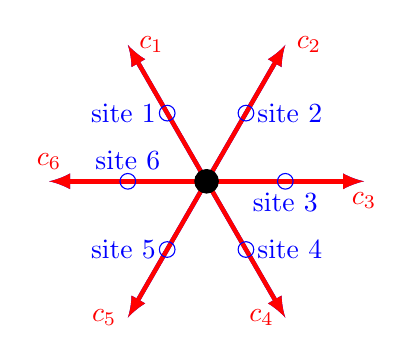
\begin{tikzpicture}

    \coordinate (Origin) at (0,0);
    \coordinate (site1) at ({2 * cos(120)}, {2 * sin(120)});
    \coordinate (site2) at ({2 * cos(60)}, {2 * sin(60)});
    \coordinate (site3) at ({2 * cos(0)}, {2 * sin(0)});
    \coordinate (site4) at ({2 * cos(-60)}, {2 * sin(-60)});
    \coordinate (site5) at ({2 * cos(-120)}, {2 * sin(-120)});
    \coordinate (site6) at ({2 * cos(-180)}, {2 * sin(-180)});
    \draw [ultra thick,-latex,blue] (Origin)
        -- (site1) node [midway, left] {site 1};
    \draw [ultra thick,-latex,blue] (Origin)
        -- (site2) node [midway, right] {site 2};
    \draw [ultra thick,-latex,blue] (Origin)
        -- (site3) node [midway, below] {site 3};
    \draw [ultra thick,-latex,blue] (Origin)
        -- (site4) node [midway, right] {site 4};
    \draw [ultra thick,-latex,blue] (Origin)
        -- (site5) node [midway, left] {site 5};
    \draw [ultra thick,-latex,blue] (Origin)
        -- (site6) node [midway, above] {site 6};     
	\draw [ultra thick,-latex,red] (Origin)
        -- (site1) node [right] {$c_1$};
    \draw [ultra thick,-latex,red] (Origin)
        -- (site2) node [right] {$c_2$};
    \draw [ultra thick,-latex,red] (Origin)
        -- (site3) node [below] {$c_3$};
    \draw [ultra thick,-latex,red] (Origin)
        -- (site4) node [left] {$c_4$};
    \draw [ultra thick,-latex,red] (Origin)
        -- (site5) node [left] {$c_5$};
    \draw [ultra thick,-latex,red] (Origin)
        -- (site6) node [above] {$c_6$};    
    \coordinate (site1) at ({ cos(120)}, { sin(120)});
    \coordinate (site2) at ({ cos(60)}, { sin(60)});
    \coordinate (site3) at ({ cos(0)}, { sin(0)});
    \coordinate (site4) at ({ cos(-60)}, { sin(-60)});
    \coordinate (site5) at ({ cos(-120)}, { sin(-120)});
    \coordinate (site6) at ({ cos(-180)}, { sin(-180)});
       
    \node[draw,circle,inner sep=3pt,fill] at (0,0) {};
    \node[draw,circle,inner sep=2pt,blue] at (site1) {};
    \node[draw,circle,inner sep=2pt,blue] at (site2) {};
    \node[draw,circle,inner sep=2pt,blue] at (site3) {};
    \node[draw,circle,inner sep=2pt,blue] at (site4) {};
    \node[draw,circle,inner sep=2pt,blue] at (site5) {};
    \node[draw,circle,inner sep=2pt,blue] at (site6) {};

  \end{tikzpicture}
  \caption{Here is an example of a single hexagonal cell with 6 velocity vectors and 6 empty sites.}
  \label{figure:Hsingle-cell}
\end{figure}
\noindent The velocity vectors must have a symmetrical property i.e. $\sum_{i = 1}^{6} \textbf{c}_{i} = \textbf{0}$. Also each vector should be of unit length. All the particles must have the same mass.
\subsubsection{Collision rules}
One difference 
\subsubsection{Propagation rules}
\subsubsection{Mass and Momentum Densities}
\subsubsection{Time complexity analysis}
\subsubsection{Applications}
\subsubsection{defects}
\subsection{\Acrfull{lbm}}
\subsubsection{History}
\subsubsection{Assumptions}
\subsubsection{Collision rules}
\subsubsection{Propagation rules}
\subsubsection{Mass and Momentum Densities}
\subsubsection{Time complexity analysis}
\subsubsection{Applications}
\subsubsection{defects}
\end{document}